\section{Benchmarking} \label{sec:benchmarking_konzepte}
\subsection{Konzepte} \label{sec:konzepte}
Die Entscheidung für ein bestimmtes \ac{llm} in der breiten Palette der verfügbaren Modelle und Anwendungsbereiche, wie in Kapitel 2 diskutiert, verlangt nach einem systematischen Ansatz. Dieser sollte die Auswahl eines geeigneten Modells basierend auf detaillierter Bewertung spezifischer Anforderungen, Leistungsmetriken und des jeweiligen Einsatzgebiets erleichtern. In der Forschung wird daher auf Benchmarking zurückgegriffen, um Modelle anhand verschiedener Kriterien zu vergleichen. Laut Kounev u.a. ist Benchmarking ein Ansatz, der Methoden und Werkzeuge zur Beurteilung und zum Vergleich von Systemen oder Komponenten in Bezug auf Leistung, Energieeffizienz, Zuverlässigkeit und Sicherheit bietet \footcite[Vgl.][S. 9]{kounev2020systems}.

Die Leistung von \acp{llm} wird in einer Vielzahl von Kontexten gemessen, darunter Dialogsysteme, maschinelle Übersetzung und Mathematik \footcites[Vgl.][S. 24]{naveed2023comprehensive} [Vgl.][S. 7 ff.]{chang2023survey}. Dabei orientiert man sich oft an den Vorgaben von \ac{helm} \footcite[Vgl.][S. 27 ff.]{liang2023holistic}. Ein wichtiges Kriterium hierbei ist die Genauigkeit. Um den Übergang von der allgemeinen Genauigkeit zu spezifischeren Metriken wie dem F1-Score zu verdeutlichen, wird nun ein Beispiel herangezogen.

Der F1-Score ist ein nützliches Maß, um die Balance zwischen Präzision und Recall zu bewerten, besonders in Fällen, wo beides wichtig ist. Ein praxisnahes Beispiel dafür ist die medizinische Diagnose. Hier wird ein Klassifikationsmodell verwendet, um gesunde von kranken Patienten zu unterscheiden. In einem Test mit 100 Patienten ergeben sich folgende Werte:

\begin{itemize}
    \item Wahre positive Vorhersagen (TP): 25
    \item Falsch positive Vorhersagen (FP): 5
    \item Falsch negative Vorhersagen (FN): 10
    \item Wahre negative Vorhersagen (TN): 60
\end{itemize}

Die Präzision, also der Anteil der korrekt identifizierten kranken Patienten unter den als krank klassifizierten, berechnet sich so\footcite[Vgl.][S. 262 f.]{derczynski-2016-complementarity}:

\begin{equation}
    \text{Präzision} = \frac{TP}{TP + FP} = \frac{25}{30} = 0.8333
\end{equation}

Der Recall, der Prozentsatz der korrekt erkannten kranken Patienten, wird wie folgt berechnet:

\begin{equation}
    \text{Recall} = \frac{TP}{TP + FN} = \frac{25}{35} \approx 0.7143
\end{equation}

Der F1-Score, der ein harmonisiertes Maß für Präzision und Recall ist, ergibt sich daraus zu:

\begin{equation}
    F1\text{-}Score = 2 \cdot \frac{\text{Präzision} \cdot \text{Recall}}{\text{Präzision} + \text{Recall}} \approx 0.7692
\end{equation}

Mit einem F1-Score von ungefähr 0.7692 zeigt das Modell eine gute Balance zwischen Präzision und Recall, was für zuverlässige Diagnosen in der medizinischen Praxis spricht.

Ein weiter Ansatz um \acp{llm} zu evaluieren ist der Einsatz menschlicher Kontrolle \footcite[Vgl.][S. 1]{chiang2023large}.
Sie ermöglicht eine qualitative Einschätzung der Textqualität, Kohärenz und Relevanz, und zwar oft im Vergleich zu Referenztexten.
Diese menschliche Bewertung kann mithilfe von Crowd-Sourcing oder Expertenbewertungen durchgeführt werden.
Ergänzend zur menschlichen Bewertung, die qualitative Aspekte wie Textqualität, Kohärenz und Relevanz im Vergleich zu Referenztexten beurteilt \footcite[Vgl.][S. 73]{liang2023holistic}, existieren weitere facettenreiche Methoden zur Evaluation von \acp{llm}.
Automatisierte Metriken wie BLEU für maschinelle Übersetzungen, ROUGE für Zusammenfassungen oder BERT für allgemein Textgenerierung \footcite[Vgl.][S. 1]{zhang2020bertscore} bieten objektive und schnell ermittelbare Ergebnisse, obwohl sie manchmal Nuancen menschlicher Sprache nicht vollständig erfassen können \footcite[Vgl.][S. 27 f.]{chang2023survey}. Die Robustheit von \acp{llm} wird häufig durch Tests mit manipulierten oder herausfordernden Eingaben überprüft, um ihre Widerstandsfähigkeit gegenüber Fehlern oder unerwarteten Daten zu beurteilen \footcite[Vgl.][S. 29 f.]{liang2023holistic}.
Ein weiterer wichtiger Aspekt ist die Überprüfung der Fairness und des Bias in \acp{llm}.
Dies umfasst spezielle Untersuchungen, um systematische Verzerrungen gegenüber verschiedenen demografischen Gruppen aufzudecken \footcite[Vgl.][S. 30 f.]{liang2023holistic}.
Auch die Bewertung der Skalierbarkeit und Effizienz, also wie gut ein Modell unter verschiedenen Hardware-Konfigurationen und bei unterschiedlichen Datengrößen funktioniert, ist von Bedeutung.
Dies schließt die Analyse von Antwortzeiten und Ressourcenverbrauch bei steigenden Anforderungen ein. \footcite[Vgl.][S. 33]{liang2023holistic}

Schließlich sind Langzeitstudien entscheidend, um zu beobachten, wie gut ein Modell mit der Evolution der Sprache und sich ändernden Anwendungskontexten zurechtkommt. Da Sprachmodelle regelmäßig aktualisiert und an neue Daten angepasst werden müssen, bietet eine langfristige Betrachtung wertvolle Einblicke in die Anpassungsfähigkeit und Nachhaltigkeit des Modells.

\subsection{Relevante Benchmarks} \label{sec:exbenchmarks}
Nachdem die verschiedenen Metriken zur Evaluation von \acp{llm} erläutert wurden, ist es nun wichtig, sich auf Benchmarks zu konzentrieren, die diese Metriken in ihrer Analyse einbeziehen.

Einer der bekanntesten Benchmarks in diesem Bereich ist der GLUE (General Language Understanding Evaluation) Benchmark \footcite[Vgl.][S. 1]{wang2019glue}.
GLUE besteht aus einer Sammlung von Tests, die darauf abzielen, das allgemeine Sprachverständnis zu messen.
Dieser Benchmark beinhaltet Aufgaben wie Textverständnis, Inferenz und die Fähigkeit, die Stimmung eines Textes zu erkennen.

Ein weiterer bedeutender Benchmark ist der SuperGLUE Benchmark, der als Nachfolger von GLUE entwickelt wurde \footcite[Vgl.][S. 1]{sarlin2020superglue}.
SuperGLUE enthält anspruchsvollere Aufgaben und zielt darauf ab, die Grenzen der neuesten Sprachmodelle zu testen. Dazu gehören komplexere Frage-Antwort-Aufgaben und die Fähigkeit, logische Schlüsse aus Texten zu ziehen.

Für spezifischere Anwendungen gibt es Benchmarks wie SQuAD (Stanford Question Answering Dataset) \footcite[Vgl.][S. 1]{rajpurkar2016squad} für Frage-Antwort-Systeme und WMT (Workshop on Machine Translation) \footcite[Vgl.][S. 1]{birch2018findings} für maschinelle Übersetzung.
SQuAD testet die Fähigkeit von Modellen, präzise Antworten auf Fragen zu geben, die auf Textpassagen basieren, während WMT die Qualität von Übersetzungen in verschiedenen Sprachpaaren bewertet.

Im Bereich der Robustheit und Fairness ist der Winogrande-Schema-Benchmark \footcite[Vgl.][S. 1]{sakaguchi2019winogrande} erwähnenswert. Dieser Benchmark konzentriert sich auf die Fähigkeit von \acp{llm}, subtile sprachliche Unterschiede und Ambiguitäten zu erkennen, was entscheidend für die Bewertung der Feinheiten menschlicher Sprache ist.



Diese Benchmarks bieten eine umfassende und vielschichtige Bewertung der Leistung von \acp{llm}. Sie ermöglichen nicht nur einen Vergleich zwischen verschiedenen Modellen, sondern bieten auch Einsichten, die zur Weiterentwicklung und Verbesserung dieser Technologien beitragen. Durch die ständige Weiterentwicklung dieser Benchmarks wird sichergestellt, dass sie mit den Fortschritten in der Sprachmodellierung Schritt halten und weiterhin relevante und aussagekräftige Ergebnisse liefern.

\subsection{Problematiken und Herausforderungen} \label{sec:problematiken}

Die Verwendung von Benchmarks zur Bewertung von \acp{llm} ist zwar unerlässlich, aber sie bringt verschiedene Herausforderungen und Problematiken mit sich, die ihre Wirksamkeit und Aussagekraft beeinträchtigen können. Eine der Hauptproblematiken ist die Überanpassung an spezifische Aufgaben \footcite[Vgl.][S. 6]{zhou2023dont}. Entwickler könnten ihre Modelle besonders auf die in den Benchmarks gestellten Aufgaben trainieren, was zu einer hohen Leistung in diesen Tests, aber nicht unbedingt zu einer guten allgemeinen Sprachverarbeitungsfähigkeit führt.
Daher wurde beispielsweise beim BIG-bench Benchmark eine sogenannte Canary-ID in den Fragen hinterlegt.
Wenn ein Sprachmodell diese ID erkennt, so weiß man, dass das Modell auf der Frage trainiert wurde \footcite[Vgl.][S. 11]{srivastava2023imitation}.

Hinzu kommt die mangelnde Repräsentativität vieler Benchmarks, die sich oft auf eine begrenzte Anzahl von Aufgaben konzentrieren und dadurch wichtige Anwendungsbereiche oder Sprachvarianten vernachlässigen können. Dies führt zu einer eingeschränkten Einschätzung der Modellleistung. Weiterhin können Benchmarks unbewusst Verzerrungen enthalten, die sich aus den verwendeten Daten oder Testbedingungen ergeben. Dies kann dazu führen, dass Modelle, die in Benchmarks gut abschneiden, in realen Anwendungsfällen, insbesondere in Bezug auf Fairness und Unvoreingenommenheit, nicht gut funktionieren.

Ein weiteres Problem ist die dynamische Natur der Sprache. Sprache entwickelt sich ständig weiter, und Benchmarks, die auf veralteten oder begrenzten Daten basieren, könnten nicht in der Lage sein, die Leistung von Modellen in Bezug auf aktuelle oder zukünftige sprachliche Trends genau zu bewerten. Zudem neigen Benchmarks dazu, sich auf leicht quantifizierbare Metriken wie Genauigkeit oder F1-Score zu konzentrieren und erfassen möglicherweise nicht qualitative Aspekte wie Sprachkreativität, Emotionalität oder den kulturellen Kontext der Sprachverwendung.

Die Komplexität und die Kosten, die mit der Durchführung umfassender Benchmarks verbunden sind, können ebenfalls ein Hindernis darstellen, insbesondere für kleinere Organisationen oder Forschungsgruppen. Schließlich ist die schnelle Entwicklung von \acp{llm} zu berücksichtigen. Da sich die Technologie hinter \acp{llm} rasant weiterentwickelt, könnten Benchmarks schnell veralten und somit keine relevanten Informationen über die neuesten Modelle bereitstellen.
Dies wird in Abbildung \ref{fig:benchmarks} deutlich, die die durchschnittliche Lebensdauer von Benchmarks zeigt.

\begin{figure}
    \centering
    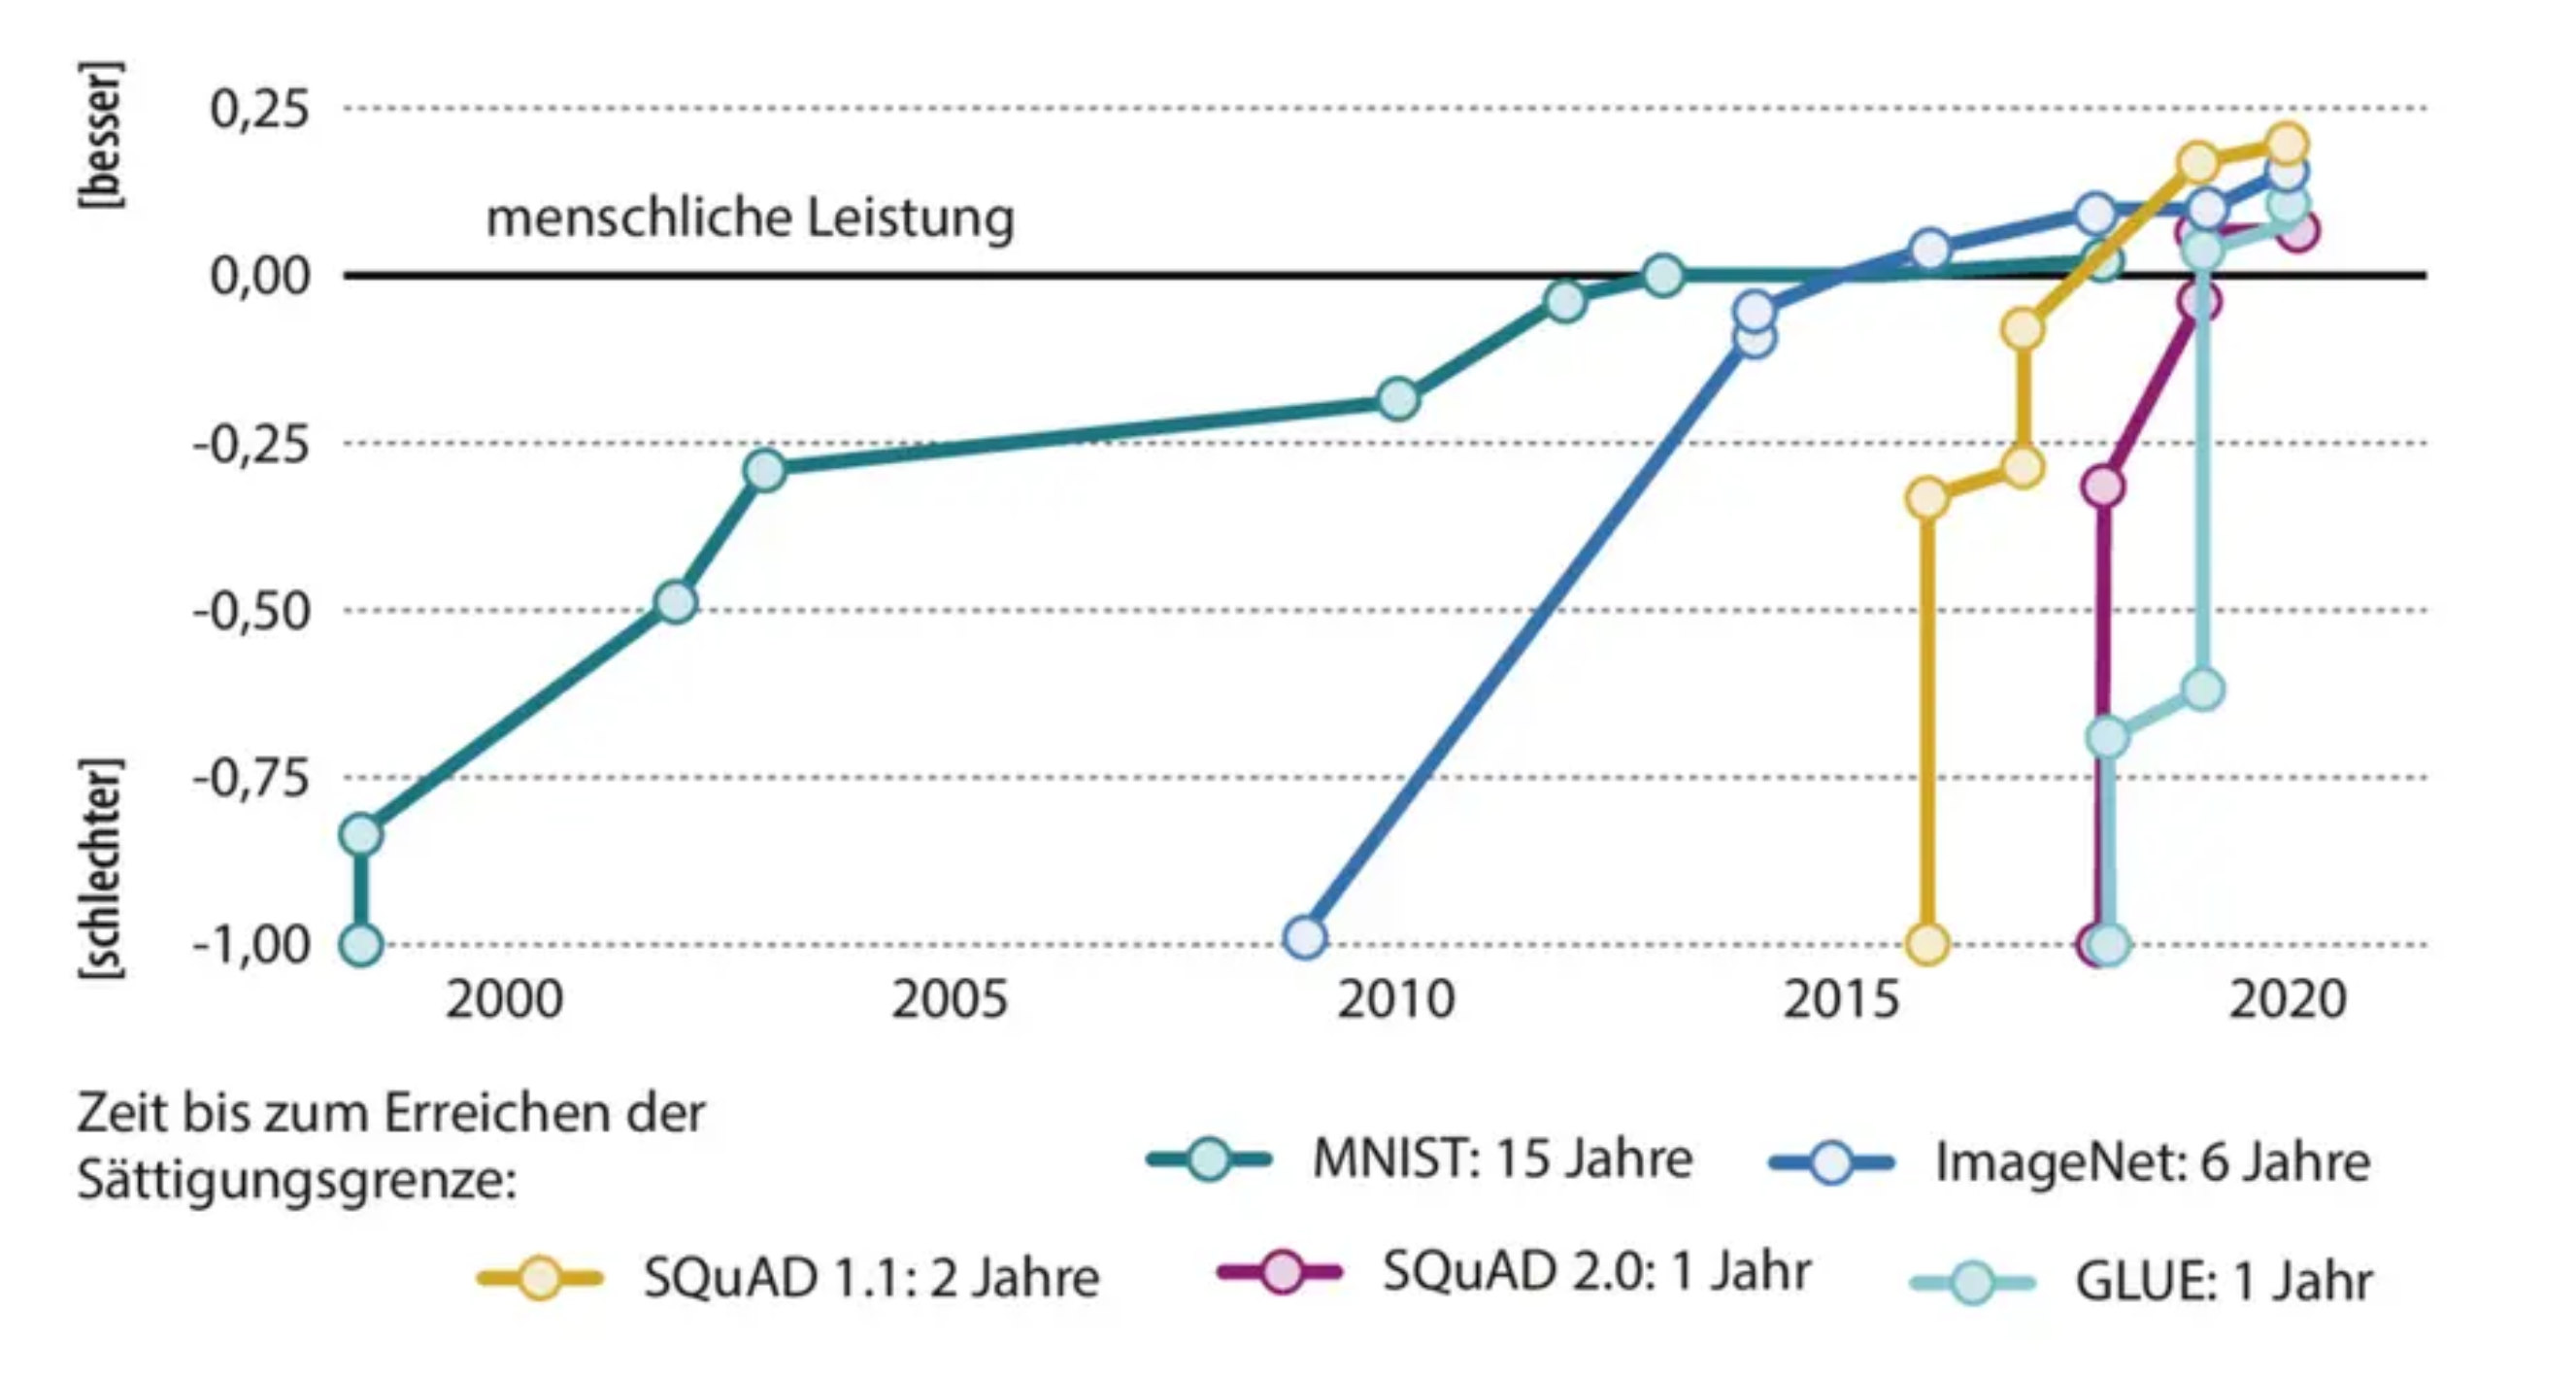
\includegraphics[width=\textwidth]{Grafiken/Lebensdauer von KI-Benchmarks.png}
    \caption{Lebensdauer von KI-Benchmarks \footcite[][S. 4]{Heise:KI}}
    \label{fig:benchmarks}
\end{figure}

Hier ist zu erkennen, dass die Lebensdauer von Benchmarks in den letzten Jahren deutlich gesunken ist, da die Entwicklung von \acp{llm} immer schneller voranschreitet.

Diese Herausforderungen machen deutlich, dass Benchmarks zwar nützliche Werkzeuge sind, aber auch sorgfältig entwickelt und regelmäßig aktualisiert werden müssen, um ihre Relevanz und Effektivität bei der Bewertung von \acp{llm} zu gewährleisten. Es ist wichtig, dass Entwickler und Forscher diese Einschränkungen erkennen und berücksichtigen, um ein vollständiges und genaues Bild der Leistungsfähigkeit und Anwendbarkeit von Sprachmodellen zu erhalten.

